%\documentclass{article}


%\usepackage{hyperref, float, amsmath} 
%\usepackage{tikz, ifthen, xcolor}
%\usepackage[english]{babel}

%\usetikzlibrary{fit, calc, arrows, shapes}

%\newcommand{\red}[1]{{\color{red} #1}}


%\begin{document}


\section{Coherence and Contexts}
\label{section:coherence}

%In general case, the coherence is established over \emph{information graphs}.

Within an agent, the coherence is established over \emph{information graphs},
containing the assessed candidate's classes and \emph{context-specific
  knowledge} --- an \emph{information graph}, that holds the information,
already known/accepted by the agent.


A \emph{context} represents an aspect for optimization/restriction, considered
by an agent. It defines context-specific information and relations over the
information graph, with the corresponding combination functions. There are
two types of relations: \emph{binary} and over the \emph{whole graph}. The former ones
are applied to every pair of nodes and the results are combined by 
\emph{binary fold functions} (one combines the results of the same relation
and the other combines the latter results). The whole-graph relations' values are
combined by the corresponding \emph{whole-graph fold function}. In the end the
combined values of both relations types are merged into the result by
\emph{combined merge function}. All the combination functions are defined at
contexts.

A candidate is propagated through the contexts in the established
order. At each context it gets assessed and the result is compared
against \emph{context-specific threshold}. If passing threshold test,
the candidate is sent to the next context, otherwise it is marked as failed
(providing a reason) and is propagated no further. In both cases the coherence
value is guarded alongside the candidate.

Some contexts are also capable of splitting a graph into acceptable
sub-graphs, as described in \cite{UAB-Thesis}.
 

\begin{figure}[H]
  \centering
  \fbox{ \input{../src/Document/tikz/ContextAssess} }
  \caption{Binary relations within an information graph. One can
           distinguish the relations between the assessed information pieces
           and the relations between assessed and the known ones.
          }
\end{figure}


\subsection{Internal Contexts}

An internal context requires no knowledge from other agents.

\subsubsection{Capabilities}

Represent \emph{strong} restrictions, imposed by the institution.

Institution restrictions:
\begin{itemize}
\item \textbf{Group:} the candidate has the correct amount of classes for each
  discipline inscribed.
\item \textbf{Professor:} can teach every discipline assigned.
\item \textbf{Classroom:} has enough capacity and meets all special requirements.
\end{itemize}

An agent should be keeping the capabilities of known agents, to avoid creation
of unacceptable classes.

\begin{figure}[H]
  \centering
  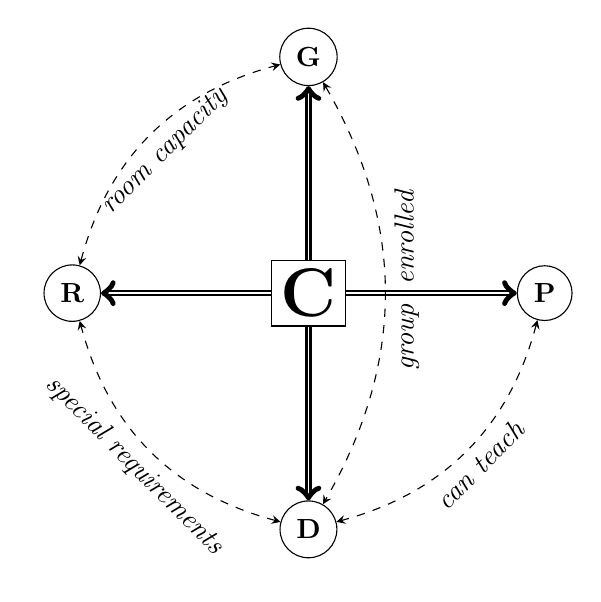
\begin{tikzpicture}

\edef\r{3cm}

\node[draw]         (C) at (0,  0) {\textbf{\Huge C}};
\node[draw, circle] (G) at (0, \r) {\textbf{G}};
\node[draw, circle] (P) at (\r, 0) {\textbf{P}};
\node[draw, circle] (D) at (0,-\r) {\textbf{D}};
\node[draw, circle] (R) at (-\r,0) {\textbf{R}};

\foreach \i in {(G),(P),(D),(R)}
 \draw[->, thick, double] (C) -- \i;

\def\data{ P/D/can teach
         , D/R/special requirements
         , R/G/room capacity
         , G/D/\quad group~~enrolled
         }

\foreach \i/\j/\k in \data
 \draw[<->, >=stealth, dashed] (\i) to[bend left
                                      ,edge node={node [sloped, below] {\emph{\k}}}]
                               (\j);


\end{tikzpicture}

  \caption{Capabilities required to form a \emph{class}.}
  \label{fig:capabilities}
\end{figure}


\subsubsection{Beliefs (Time Consistency)}

Asserts that all the classes (concerning the assessing agent), are consistent in
time (do not intersect). This context is a splitting one, it uses the time
consistence relation to generate all possible time-consistent candidates from
given classes. It's internal knowledge should hold \emph{classes pool}, that
would be used for candidates generation via \emph{graph splitting}.

\red{todo: 

  images from g-drive: ``Graph Coherence Assessment Examples''
  and ``Coherence Graph Partition - 7''

  text from ``Beliefs.lhs''

}

\subsubsection{Obligations}

\red{TO DO}

\subsubsection{Preference}

\red{TO DO}

\subsection{External}

The external context asks counterparts an \emph{opinion} about a candidate.
An opinion is the \emph{inner coherence} (coherence accumulated at internal
contexts) of the agent being asked.

\red{todo: images from g-drive ``ThesisCandidatesCommonGoal''}

%\end{document}

